\documentclass{beamer}
\usetheme{Copenhagen}
\usecolortheme{beaver}
\beamertemplatenavigationsymbolsempty
\makeatletter
\setbeamertemplate{footline}{}
\makeatother

\definecolor{unibored}{RGB}{187,46,41}
\setbeamercolor{title}{fg=unibored}
\setbeamercolor{beamercolorbox}{fg=unibored}

\setbeamertemplate{title page}{
    \vfill
    \begin{center}
        {\usebeamerfont{title}\usebeamercolor[fg]{title}\inserttitle\par}
    \end{center}

    \vfill

    \begin{center}
        {\usebeamerfont{author}\insertauthor\par}
        \vspace{0.2cm}
        {\usebeamerfont{institute}\insertinstitute\par}
        \vspace{0.5cm}
        {\usebeamerfont{date}\insertdate\par}
    \end{center}
}

\title{Merkle-tree-based integrity verification protocol for geo-distributed storage
systems}

\author{Santo Cariotti}

\institute{Alma Mater Studiorum\\ Università di Bologna}
\date{October 30, 2025}


\usepackage{listings}

\usepackage{graphicx}
\usepackage{tikz}
\usetikzlibrary{arrows.meta,positioning,calc,fit}
\usetikzlibrary{shapes.geometric}
\usepackage[ruled,linesnumbered,vlined]{algorithm2e}

\begin{document}
\frame{\titlepage}

\begin{frame}{Content}

\begin{enumerate}
    \item What problem are we addressing?
    \item How did we solve it?
    \item What about scalability?
\end{enumerate}

\end{frame}

\begin{frame}{Problem}
Given a filesystem, how can I be sure that every file keeps integrity?

\begin{center}
    \begin{tikzpicture}
        % 1. Include your image in a node
        \node[anchor=south west,inner sep=0] (image) at (0,0) {
            \includegraphics[width=0.8\linewidth]{static/shell-ls-problem.png}
        };

        % Calculate the width and height of the image node for later use
        \pgfgetlastxy{\imagewidth}{\imageheight}

        \only<2>{
            \coordinate (A) at ([xshift=.7cm, yshift=2.1cm]image.south west);
            \coordinate (B) at ([xshift=7.9cm, yshift=2.4cm]image.south west);

            \draw[red, very thick, line width=1pt]
                (A) rectangle (B);
        }
    \end{tikzpicture}
\end{center}

\only<2>{We could use a checksum system to find out that the bordered file is
corrupted.}

\end{frame}

\begin{frame}{Problem}
    \begin{columns}[c]
        \begin{column}{0.4\textwidth}
            But, if we have more than one filesystem distributed across
            different regions?
            \only<2->{We should make a checksum check for each node.}
            \only<3>{\textcolor{red}{\textbf{Too complex.}}}
        \end{column}
        \begin{column}{0.6\textwidth}

            \begin{tikzpicture}
                \draw[thick] (0,0) rectangle (4,3);
                \node[anchor=north west] at (0,3) {\textbf{Switzerland}};
                \node[circle, draw, thick, minimum size=1.5cm] at (1,1) {node4};
                \node[circle, draw, thick, minimum size=1.5cm] at (3,1) {node5};

                \draw[thick] (0,4) rectangle (6,7);
                \node[anchor=north west] at (0,7) {\textbf{Italy}};
                \node[circle, draw, thick, minimum size=1.5cm] at (1,5.5) {node1};
                \only<1>{
                    \node[circle, draw, thick, minimum size=1.5cm] at (3,5.5) {node2};
                }
                \only<2->{
                    \node[circle, draw, red, densely dotted, thick, minimum size=1.5cm] at (3,5.5) {node2};
                }
                \node[circle, draw, thick, minimum size=1.5cm] at (5,5.5) {node3};
            \end{tikzpicture}
        \end{column}
    \end{columns}
\end{frame}

\begin{frame}{Cubbit}
\centering
\includegraphics[width=0.4\linewidth]{static/cubbit-logo.png}
\\
\vspace{1em}
Cubbit, a geo-distributed storage system.\\
\end{frame}

\begin{frame}{Cubbit -- How it works}
    \begin{columns}[c]
        \begin{column}{0.4\textwidth}
            Each file is split in $n+k$ shards (i.e., pieces). \\ At least $n$ shards are
            required to reconstruct the file, while $k$ shards provide redundancy.
        \end{column}
        \begin{column}{0.6\textwidth}

            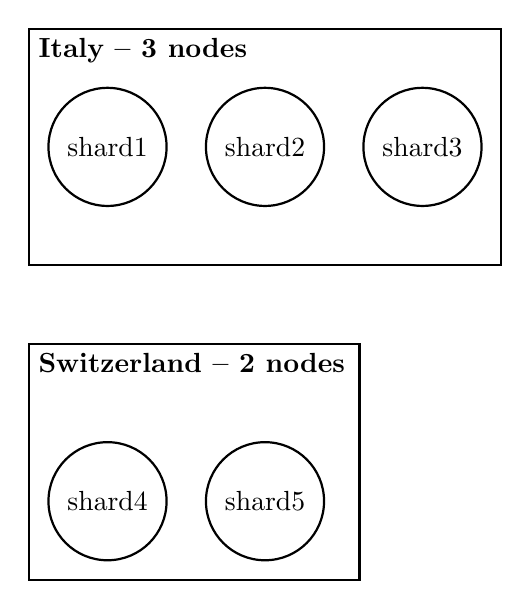
\begin{tikzpicture}
                \draw[thick] (0,0) rectangle (4.2,3);
                \node[anchor=north west] at (0,3) {\textbf{Switzerland -- 2 nodes}};
                \node[circle, draw, thick, minimum size=1.5cm] at (1,1) {shard4};
                \node[circle, draw, thick, minimum size=1.5cm] at (3,1) {shard5};

                \draw[thick] (0,4) rectangle (6,7);
                \node[anchor=north west] at (0,7) {\textbf{Italy -- 3 nodes}};
                \node[circle, draw, thick, minimum size=1.5cm] at (1,5.5) {shard1};
                \node[circle, draw, thick, minimum size=1.5cm] at (3,5.5) {shard2};
                \node[circle, draw, thick, minimum size=1.5cm] at (5,5.5) {shard3};
            \end{tikzpicture}
        \end{column}
    \end{columns}
\end{frame}

\begin{frame}{Cubbit -- Problems using checksum}
    \begin{columns}[c]
        \begin{column}{0.4\textwidth}
            \begin{enumerate}
                \item<1-> If nodes are offline, it becomes impossible to check all shards for a file.
                \item<2-> During an upload some agents can be offline, but they
                could be online during the check.
                \item<3-> Check for each reconstructed file or for each shard?
            \end{enumerate}

        \end{column}
        \begin{column}{0.6\textwidth}

            \begin{tikzpicture}
                \draw[thick] (0,0) rectangle (4.2,3);
                \node[anchor=north west] at (0,3) {\textbf{Switzerland -- 2 nodes}};
                \node[circle, draw, dotted, minimum size=1.5cm] at (1,1) {shard4};
                \node[circle, draw, dotted, minimum size=1.5cm] at (1,1) {shard4};
                \node[circle, draw, thick, minimum size=1.5cm] at (3,1) {shard5};

                \draw[thick] (0,4) rectangle (6,7);
                \node[anchor=north west] at (0,7) {\textbf{Italy -- 3 nodes}};
                \node[circle, draw, thick, minimum size=1.5cm] at (1,5.5) {shard1};
                \only<1>{\node[circle, draw, thick, minimum size=1.5cm] at (3,5.5) {shard2};}
                \only<2->{\node[circle, draw, thick, minimum size=1.5cm] at
                (3,5.5) {n/a};}
                \node[circle, draw, dotted, minimum size=1.5cm] at (5,5.5) {shard3};
            \end{tikzpicture}
        \end{column}
    \end{columns}
\end{frame}

\begin{frame}
    \usebeamerfont{title}\usebeamercolor[fg]{title}Solution\par
\end{frame}

\begin{frame}{Solution}

Each node uses a Merkle-tree-structure to organize shards during the integrity
verification. Every node agree on what file is corrupted thanks to Raft. Data
    are organized using Reed-Solomon codes.

\begin{center}
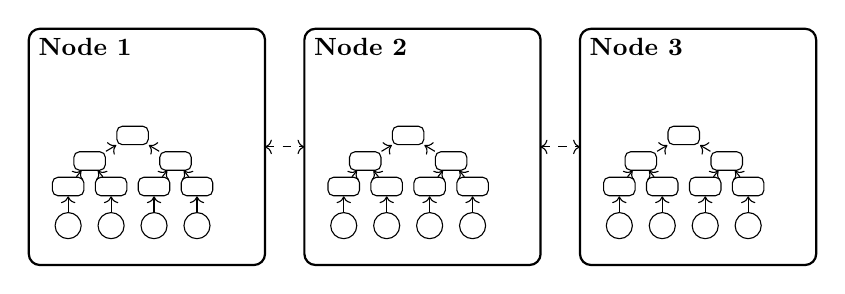
\begin{tikzpicture}[
    % Base styles for the small trees
    every node/.style={font=\small},
    leaf/.style={draw, circle, minimum size=2mm},
    hash/.style={draw, rectangle, rounded corners=2pt,
        minimum width=4mm, minimum height=2mm, % Increased size slightly
        sibling distance=1cm,
        align=center},
    node distance=2mm, % Increased distance slightly
    % Main positioning for the large blocks (not used as nodes, but kept)
    block/.style={draw, thick, rounded corners, inner sep=12pt}
]

% ==================== BLOCK 1: NODE 1 ====================
\begin{scope}[xshift=0cm]
    % leaves
    \node[leaf,] (d1-0) {};
    \node[leaf, right=of d1-0] (d1-1) {};
    \node[leaf, right=of d1-1] (d1-2) {};
    \node[leaf, right=of d1-2] (d1-3) {};
    % leaf-hash nodes
    \node[hash, above=0.2cm of d1-0] (n1-0) {};
    \node[hash, above=0.2cm of d1-1] (n1-1) {};
    \node[hash, above=0.2cm of d1-2] (n1-2) {};
    \node[hash, above=0.2cm of d1-3] (n1-3) {};
    % parents
    \node[hash, above=of $(n1-0)!0.5!(n1-1)$] (p1-01) {};
    \node[hash, above=of $(n1-2)!0.5!(n1-3)$] (p1-23) {};
    % root
    \node[hash, above=of $(p1-01)!0.5!(p1-23)$] (root1) {};
    % edges with arrows
    \foreach \a/\b in {d1-0/n1-0, d1-1/n1-1, d1-2/n1-2, d1-3/n1-3, n1-0/p1-01, n1-1/p1-01, n1-2/p1-23, n1-3/p1-23, p1-01/root1, p1-23/root1}
        \draw[->] (\a) -- (\b);

    % Explicitly drawn rectangle and label
    \draw[thick, rounded corners] (-0.5,-0.5) rectangle (2.5,2.5);
    \node[anchor=north west] at (-0.5,2.5) {\textbf{Node 1}};
    % Define coordinates for connection (center of the right edge)
    \coordinate (East1) at (2.5, 1.0); 
\end{scope}

% ==================== BLOCK 2: NODE 2 ====================
\begin{scope}[shift=({3.5cm, 0cm})]
    % leaves
    \node[leaf,] (d2-0) {};
    \node[leaf, right=of d2-0] (d2-1) {};
    \node[leaf, right=of d2-1] (d2-2) {};
    \node[leaf, right=of d2-2] (d2-3) {};
    % leaf-hash nodes
    \node[hash, above=0.2cm of d2-0] (n2-0) {};
    \node[hash, above=0.2cm of d2-1] (n2-1) {};
    \node[hash, above=0.2cm of d2-2] (n2-2) {};
    \node[hash, above=0.2cm of d2-3] (n2-3) {};
    % parents
    \node[hash, above=of $(n2-0)!0.5!(n2-1)$] (p2-01) {};
    \node[hash, above=of $(n2-2)!0.5!(n2-3)$] (p2-23) {};
    % root
    \node[hash, above=of $(p2-01)!0.5!(p2-23)$] (root2) {};
    % edges with arrows
    \foreach \a/\b in {d2-0/n2-0, d2-1/n2-1, d2-2/n2-2, d2-3/n2-3, n2-0/p2-01, n2-1/p2-01, n2-2/p2-23, n2-3/p2-23, p2-01/root2, p2-23/root2}
        \draw[->] (\a) -- (\b);

    % Explicitly drawn rectangle and label
    \draw[thick, rounded corners] (-0.5,-0.5) rectangle (2.5,2.5);
    \node[anchor=north west] at (-0.5,2.5) {\textbf{Node 2}};
    % Define coordinates for connection
    \coordinate (West2) at (-0.5, 1.0); % Left side center
    \coordinate (East2) at (2.5, 1.0);  % Right side center
\end{scope}

% ==================== BLOCK 3: NODE 3 ====================
\begin{scope}[shift=({7cm, 0cm})]
    % leaves
    \node[leaf,] (d3-0) {};
    \node[leaf, right=of d3-0] (d3-1) {};
    \node[leaf, right=of d3-1] (d3-2) {};
    \node[leaf, right=of d3-2] (d3-3) {};
    % leaf-hash nodes
    \node[hash, above=0.2cm of d3-0] (n3-0) {};
    \node[hash, above=0.2cm of d3-1] (n3-1) {};
    \node[hash, above=0.2cm of d3-2] (n3-2) {};
    \node[hash, above=0.2cm of d3-3] (n3-3) {};
    % parents
    \node[hash, above=of $(n3-0)!0.5!(n3-1)$] (p3-01) {};
    \node[hash, above=of $(n3-2)!0.5!(n3-3)$] (p3-23) {};
    % root
    \node[hash, above=of $(p3-01)!0.5!(p3-23)$] (root3) {};
    % edges with arrows
    \foreach \a/\b in {d3-0/n3-0, d3-1/n3-1, d3-2/n3-2, d3-3/n3-3, n3-0/p3-01, n3-1/p3-01, n3-2/p3-23, n3-3/p3-23, p3-01/root3, p3-23/root3}
        \draw[->] (\a) -- (\b);

    % Explicitly drawn rectangle and label
    \draw[thick, rounded corners] (-0.5,-0.5) rectangle (2.5,2.5);
    \node[anchor=north west] at (-0.5,2.5) {\textbf{Node 3}};
    % Define coordinates for connection
    \coordinate (West3) at (-0.5, 1.0); % Left side center
\end{scope}

% ==================== CONNECTIONS BETWEEN RECTANGLES ====================
% The coordinates are defined as global coordinates, so they can be referenced directly.
% Connection 1-2
\draw[<->, dashed] (East1) -- (West2);

% Connection 2-3
\draw[<->, dashed] (East2) -- (West3);

\end{tikzpicture}
\end{center}

\end{frame}


\chapter{Background}

This chapter is intended to provide the reader with some background information on the technologies used in writing this thesis project.

Some of them are essential to better know why the given Merkle tree solution is useful and works for Cubbit's infrastructure.

\section{Merkle Trees}\label{section:merkle-trees}

Merkle trees \cite{merkle1979} are a fundamental data structure first introduced by R. Merkle in his PhD dissertation. This section presents the theoretical foundations of Merkle trees, their construction, their practical applications, and the rationale for the implementation chosen in this thesis.

A Merkle tree is a binary tree $T$ of height $H$ with $2^H$ leaves and $2^H - 1$ internal nodes.  
Each leaf stores the cryptographic hash of the underlying data, rather than the raw data itself. The same cryptographic hash function is applied recursively at internal nodes, which store the hash of the concatenation of their two children. For a more detailed discussion of collision resistance in cryptographic hash functions, see \cite{damgaard1987collision}.

Formally, given two child nodes $n_{\text{left}}$ and $n_{\text{right}}$, their parent node is defined as:
\begin{equation}
\label{equation:nparent}
    n_{\text{parent}} = f(n_{\text{left}} \, || \, n_{\text{right}})
\end{equation}
where $||$ denotes bit-string concatenation and $f$ is a cryptographic hash function.

Consider now a Merkle tree of height $H > 2$. A leaf node is indexed by $\phi \in \{0, \ldots, 2^H-1\}$. A node at height $h$ and position $j$ (counting from left to right) is denoted as $y_h[j]$, where $h = 0, \ldots, H$ and $j = 0, \ldots, 2^{H-h}-1$.  
Given a cryptographic hash function $f: \{0,1\}^\star \mapsto \{0,1\}^n$, the recursive definition of an internal node is:
\begin{equation}
    y_h[j] = f\big(y_{h-1}[2j] \, || \, y_{h-1}[2j+1]\big).
\end{equation}

The root node of the tree, known as the \emph{Merkle root}, serves as a compact commitment to all data contained in the leaves. Because hashes propagate upwards, even a single-bit modification in any leaf causes a change in the root hash. This property makes Merkle trees powerful tools for integrity verification in large, distributed datasets.


\subsection{Merkle proofs}

One of the most powerful features of Merkle trees is the ability to prove that a given piece of data is part of a larger set, without revealing or recomputing the entire dataset.  
Given a Merkle tree leaf, one can reconstruct the root by traversing the path to the root and successively combining the node with its siblings.  


\begin{figure}[h]
\centering
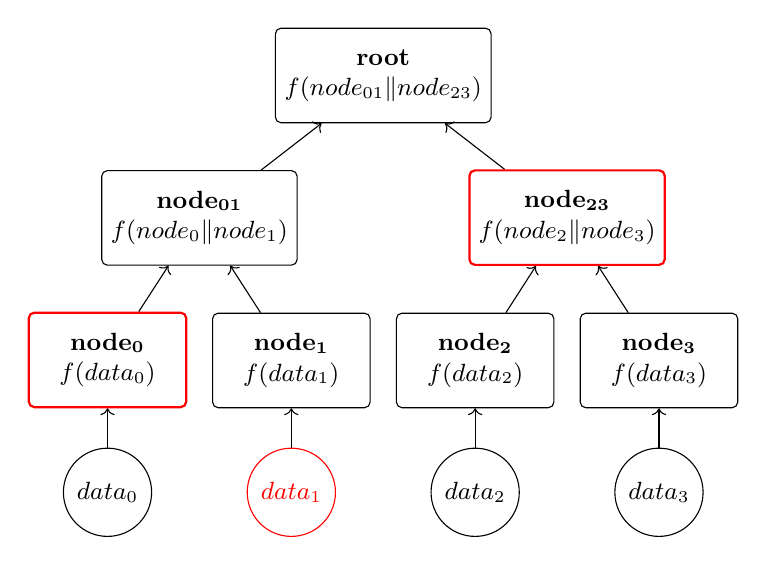
\begin{tikzpicture}[
  every node/.style={font=\small},
  leaf/.style={draw, circle, minimum size=7mm},
  hash/.style={draw, rectangle, rounded corners=2pt,
  highlight/.style={fill=yellow!40, thick},
  red/.style={draw=red, thick},
  minimum width=20mm, minimum height=12mm, 
  sibling distance=3cm,
  align=center},
  node distance=12mm
]
% leaves
\node[leaf,] (data0) {$data_0$};
\node[leaf, red, right=of data0] (data1) {$data_1$};
\node[leaf, right=of data1] (data2) {$data_2$};
\node[leaf, right=of data2] (data3) {$data_3$};
% leaf-hash nodes with two lines (inline math for each line)
\node[hash, red, above=0.5cm of data0] (n0) {\(\mathbf{node_0}\)\\ \(f(data_0)\)};
\node[hash, above=0.5cm of data1] (n1) {\(\mathbf{node_1}\)\\ \(f(data_1)\)};
\node[hash, above=0.5cm of data2] (n2) {\(\mathbf{node_2}\)\\ \(f(data_2)\)};
\node[hash, above=0.5cm of data3] (n3) {\(\mathbf{node_3}\)\\ \(f(data_3)\)};
% parents
\node[hash, above=of $(n0)!0.5!(n1)$] (p01) {\(\mathbf{node_{01}}\)\\ \(f(node_0\Vert node_1)\)};
\node[hash, red, above=of $(n2)!0.5!(n3)$] (p23) {\(\mathbf{node_{23}}\)\\ \(f(node_2\Vert node_3)\)};
% root
\node[hash, above=of $(p01)!0.5!(p23)$] (root) {\(\textbf{root}\)\\ \(f(node_{01}\Vert node_{23})\)};
% edges with arrows
\foreach \a/\b in {data0/n0, data1/n1, data2/n2, data3/n3, n0/p01, n1/p01, n2/p23, n3/p23, p01/root, p23/root}
  \draw[->] (\a) -- (\b);
\end{tikzpicture}
\caption{Merkle tree authentication path for $data_1$.  
Leaves are hashed as $node_i = f(data_i)$, and internal nodes are computed as $f(node_{\text{left}} || node_{\text{right}})$ (Equation~\ref{equation:nparent}).  
The proof requires only the sibling nodes $\{node_0, node_{23}\}$ to recompute the root.}
\label{proof-path-l1}
\end{figure}


For each height $h < H$, we define $Auth_h$ to be the value of the sibling node along the path from the leaf to the root. The set of all such siblings $\{Auth_h\}_{h=0}^{H-1}$ is called the \emph{authentication path}. With this path, anyone can recompute the root and verify inclusion by comparing against the published Merkle root.

For instance, Figure \ref{proof-path-l1} shows the authentication path corresponding to the second leaf.

This property, known as a \emph{Merkle proof}, enables efficient verification of data integrity. In a naive implementation, the entire Merkle tree is stored in memory. In such a case, generating a proof for a leaf -- as illustrated in Algorithm \ref{algo:merkle-proof-generation} -- involves traversing only the path from the leaf to the root. This reduces proof generation from a potentially linear scan of all data ($O(n)$) to a logarithmic traversal of the tree ($O(\log n)$).

\vspace{1em}
\begin{algorithm}[H]
\SetAlgoLined
\DontPrintSemicolon
\KwIn{Leaf index $i$, full tree levels $L_0, L_1, \dots, L_H$}
\KwOut{Merkle proof $\pi$ for leaf $l_i$ (or \texttt{None} if $i$ invalid)}
\BlankLine
$\pi \gets \emptyset$\;
$current \gets i$\;
\ForEach{level $\in \{L_0, \dots, L_{H-1}\}$}{
    $sibling\_index \gets \min(current \oplus 1, |level| - 1)$\;
    $sibling \gets level[sibling\_index]$\;
    $position \gets$ \texttt{Left} if $sibling\_index < current$, else \texttt{Right}\;
    append $(sibling.hash, position)$ to $\pi$\;
    $current \gets \lfloor current / 2 \rfloor$
}
\Return{$\pi$}\;
\caption{Merkle proof generation}
\label{algo:merkle-proof-generation}
\end{algorithm}

\vspace{1em}

Merkle proof verification algorithm for a proof $\pi$ is illustrated in Algorithm \ref{algo:merkle-proof-verification}.

 \vspace{1em}

\begin{algorithm}[H]
\SetAlgoLined
\DontPrintSemicolon
\KwIn{Data $d$, proof $\pi$, expected root $R$, hash function $f$}
\KwOut{\texttt{true} if valid, \texttt{false} otherwise}
\BlankLine
$h \gets f(d)$\;
\ForEach{ $(sibling, position)$ in $\pi$ }{
    \eIf{$position = \text{Left}$}{
        $h \gets f(sibling || h)$\;
    }{
        $h \gets f(h || sibling)$\;
    }
}
\Return{$h = R$}\;
\caption{Merkle proof verification}
\label{algo:merkle-proof-verification}
\end{algorithm}

\paragraph{Complexity Analysis}
\begin{itemize}
    \item \textbf{Proof generation:} $O(\log n)$, because only the sibling nodes along the path from leaf to root are collected.  
    \item \textbf{Proof verification:} $O(\log n)$, as each step requires a single hash operation per tree level.  
    \item \textbf{Memory:} $O(n)$ to store the full tree in memory, which allows logarithmic-time proof generation.
\end{itemize}

This approach ensures that Merkle proofs remain efficient even for large datasets, while keeping the implementation simple and compatible with our folder-level integrity checks across a Raft-coordinated cluster.


\subsection{Applications}

Merkle trees are widely used in distributed systems to ensure data integrity:
\begin{itemize}
    \item \textbf{Blockchains}: Bitcoin \cite{bitcoinwiki-merkle}, Ethereum \cite{ethereum-patricia}, and other systems use Merkle roots to verify transactions efficiently.
    \item \textbf{Version control systems}: Git stores commits as Merkle trees, ensuring history integrity.
    \item \textbf{Distributed storage}: Systems such as IPFS \cite{ipfs-merkle-dag} and Amazon DynamoDB \cite{decandia2007dynamo} use Merkle trees for consistency checks and conflict resolution.
\end{itemize}

\subsection{Alternative Implementations}

In the literature, several advanced variants of Merkle trees exist, such as XMSS (eXtended Merkle Signature Scheme) \cite{buchmann2011xmss} and the BDS (Buchmann-Dahmen-Szydlo) traversal algorithm \cite{buchmann2008merkle}. These schemes were developed in the context of \emph{post-quantum cryptography} and digital signatures. XMSS is standardized by the IETF (RFC 8391) and provides strong security guarantees by organizing one-time signatures (OTS) under a large Merkle tree, where the root of the tree serves as the public key.  

In XMSS, to sign a message $i$, the authentication path of the $i$-th leaf is needed. In a native way, recomputing this path would require rebuilding large parts of the tree, which becomes impractical when the tree contains millions of leaves. To solve this, the BDS traversal algorithm was introduced: it incrementally maintains and updates the authentication path in $O(h)$ time and $O(h)$ space (where $h = \log_2(n)$ is the tree height). This makes XMSS practical for very large trees.

In our case, however, the scenario is fundamentally different. We are not
designing a post-quantum signature scheme but an integrity verification protocol
for folders in a geo-distributed storage cluster. The size of our Merkle trees is modest: typically on the order of tens of leaves per folder. For trees of this size:
\begin{itemize}
    \item Proofs can be recomputed directly, without significant computational overhead.
    \item The space-time optimizations of BDS provide no practical benefit.
    \item The additional complexity of XMSS and BDS would introduce unnecessary implementation overhead.
\end{itemize}

For this reason, this thesis opted for a \emph{simple} Merkle tree implementation, applied independently at the folder and sub-folder level. This keeps the system lightweight, efficient, and easy to integrate with a consensus mechanism. It also avoids the pitfalls of managing very large Merkle trees (as in XMSS) or the stateful requirements of post-quantum signature schemes, which are irrelevant in our use case.


\section{Cryptographic Hash Functions}\label{sec:cryptopgrahic-hash-functions}

In the previous section, Merkle trees were discussed in detail, with particular attention to the use of cryptographic hash functions for node construction.  
One of the questions that emerged during my internship was: \emph{``what is the fastest cryptographic hash function?''}.  
% Although it is difficult to provide a definitive answer to this question, the Rust implementation of Merkle trees that I developed and published on \texttt{crates.io} was designed to be flexible.  
% Specifically, it relies on a trait-based abstraction that allows the integration of different hash functions depending on the desired use case.

% The current version of \texttt{mt-rs}\footnote{\url{https://crates.io/crates/mt-rs}} includes support for three hash functions: SHA-256, Keccak-256, and BLAKE3.  

This section explores the motivation behind testing different cryptographic hash functions (SHA-256, Keccak-256, and BLAKE3) within the context of this project and why, among these, BLAKE3 was selected as the primary candidate for benchmarking in this thesis due to its performance and modern design.  

\subsection{SHA-256}

SHA-256 is part of the SHA-2 family of cryptographic hash functions, standardized by NIST in 2001 \cite{penard2008secure}.
It produces a 256-bit output from input messages of arbitrary length and is widely used in security protocols such as TLS, digital signatures, and blockchain systems like Bitcoin.

The algorithm processes data in 512-bit blocks using 32-bit words. On 32-bit architectures, this design choice makes SHA-256 relatively efficient. However, on modern 64-bit CPUs, the reliance on 32-bit operations leads to extra instructions, making it slower than SHA-512 and significantly less efficient than more modern designs such as BLAKE3. By contrast, SHA-512 processes 1024-bit message blocks with 64-bit operations, making it more efficient on such architectures. In this thesis, however, SHA-512 was not benchmarked, as the focus was on SHA-256 and the comparison against Keccak-256 and BLAKE3.

Despite these performance limitations, SHA-256 remains a cornerstone in cryptography due to its simplicity, standardization, and lack of practical vulnerabilities. It is often used as a reference point in performance evaluations of newer hash functions.

\subsection{Keccak-256}

Keccak-256 \cite{bertoni2013keccak} is the 256-bit variant of the Keccak family, which won the NIST SHA-3 competition in 2012 \cite{nist-sha3}. Unlike SHA-2, Keccak is based on a \emph{sponge construction} that alternates between absorbing input blocks and squeezing output. This design provides strong theoretical guarantees and a high level of security against known cryptanalytic attacks.  

Although Keccak-256 is cryptographically very robust, its performance is generally slower than SHA-2 and significantly slower than BLAKE3 in software implementations. However, its adoption is widespread in domains where security guarantees are paramount. A prominent example is Ethereum, where Keccak-256 is used extensively in transaction validation, block hashing, and smart contract execution.  

In this thesis, Keccak-256 is included not because of raw speed but because of its relevance in production distributed systems, where it demonstrates the trade-off between cryptographic strength and computational efficiency.

\subsection{BLAKE3}

The BLAKE3 cryptographic hash function \cite{blake3-oconnor} is an evolution of the BLAKE2 cryptographic hash function \cite{aumasson2013blake2}, providing higher performance and introducing several additional features:
\begin{itemize}
    \item Support for hashing, keyed hashing, and key derivation modes.
    \item No additional space cost for keyed hashing.
    \item Parallelizable output generation.
\end{itemize}

BLAKE3 employs a binary tree structure that splits the input into 1024-byte chunks, which are treated as the leaves of the tree. The final chunk may be shorter, but it cannot be empty (unless the entire input is empty). This design enables unlimited parallelism, as each chunk can be compressed independently, allowing efficient use of modern CPUs with SIMD instructions.

BLAKE3 achieves significantly better performance than both SHA-256 and SHA-512 on modern 64-bit architectures. Within the SHA family, SHA-512 generally outperforms SHA-256 on 64-bit machines \cite{gueron2011sha}. 

BLAKE3's superior performance stems from its fundamentally different design philosophy. Unlike the inherently sequential SHA algorithms, its tree-based parallelism, fewer rounds, more efficient mixing function, and better cache locality enable it to outperform both SHA variants regardless of word size alignment considerations.

It provides a 128-bit security level and a 256-bit output.

Formally, for a message of length $n > 1024$ bytes, the left subtree covers a number of bytes equal to:

\[
2^{10 + \lfloor \log_2{\left(\frac{n-1}{1024}\right)} \rfloor}
\]

The right subtree consists of the remainder. BLAKE3 supports input of any length $0 \leq \ell < 2^{64}$.

This section does not aim to present the full specification of BLAKE3 (its compression function or operational modes) but rather to highlight its practical performance advantages.

\subsubsection{Performance}

Figures \ref{fig:blake3-thoughput-example} and \ref{fig:blak3-speed} show benchmark results from an AWS \texttt{c5.metal} instance equipped with dual Intel Xeon Platinum 8275CL (Cascade Lake-SP) processors supporting AVX-512.  
These results highlight BLAKE3's superior performance compared to other widely used hash functions.

\begin{figure}
    \centering
    \includegraphics[width=0.7\linewidth]{assets/blake3-throughput-example.png}
    \caption{Single-threaded throughput of BLAKE3 and other hash functions on an AWS c5.metal
instance, measured in cycles per byte (cpb). Lower values indicate fewer CPU cycles needed per byte.}
    \label{fig:blake3-thoughput-example}
\end{figure}

\begin{figure}
    \centering
    \includegraphics[width=0.7\linewidth]{assets/blake3-speed.png}
    \caption{Hashing speed comparison of BLAKE3 and other hash functions on an AWS c5.metal instance
with a 16~KiB input, using a single thread. Higher values (MiB/s) indicate faster processing.}
    \label{fig:blak3-speed}
\end{figure}

In the context of this thesis, benchmarks were also conducted using the \texttt{mt-rs}\footnote{\url{https://crates.io/crates/mt-rs}} library to evaluate Merkle tree creation and proof generation under these three different cryptographic hash functions.  
For each function, three tests were performed with node data sizes of 5 MB, 10 MB and 15 MB.  
In each test, the benchmark measures the time required to construct the authentication path for a leaf, verify the corresponding root from that path, and repeat this process for all 10 nodes of the Merkle tree.

The results, reported in Table \ref{tab:benchmarks-hash-functions}, demonstrate that BLAKE3 consistently outperforms both SHA-256 and Keccak-256 in terms of execution time.

\begin{table}[h!]
    \centering
    \begin{tabular}{|l|c|c|c|}
    \hline
       \textbf{Hash function} & \textbf{5 MB} & \textbf{10 MB} & \textbf{15 MB} \\
       \hline
        SHA-256 & 89.901 ms & 178.42 ms & 268.53 ms \\
        Keccak-256 & 521.49 ms & 1.1334 s & 1.3438 s \\
        BLAKE3 & 73.091 ms & 154.68 ms & 219.79 ms \\
        \hline
    \end{tabular}
    \caption{Merkle tree benchmarks with 10 nodes per dataset size (5 MB, 10 MB, and 15 MB).}
    \label{tab:benchmarks-hash-functions}
\end{table}

\section{Consensus Protocols}

This section provides background on the consensus protocols that were studied
during the internship in order to evaluate how to integrate this Merkle-tree-based integrity verification protocol into a distributed setting.  
Although corruption detection could be applied in a centralized environment using simple checksums, in a distributed cluster, a consensus algorithm is needed to coordinate nodes and ensure consistent state.  

Several consensus mechanisms were examined, reflecting the long-standing debate between \emph{leader-based} protocols (such as Raft, PBFT, and PB-Raft) and \emph{leaderless} approaches (such as Flutter+Blink). Each design choice has implications for performance, fault tolerance, and implementation complexity.

\subsection{Raft} \label{sec:raft}

Raft \cite{raft} is a consensus protocol designed to be understandable and practical, and it has become widely adopted in distributed systems such as \texttt{etcd} \cite{etcd-raft} and TiKV \cite{tikv-raft}.
It tolerates \emph{crash faults}, but not Byzantine behaviour \cite{lamport1972byzantine}.

Each server on a Raft cluster is modelled as a finite state machine with three possible states:
\begin{itemize}
    \item \textbf{Follower:} Passive state that responds to requests from the leader and candidates.
    \item \textbf{Candidate:} Initiates an election when a follower times out without hearing from a leader.
    \item \textbf{Leader:} Elected through majority vote, responsible for handling client requests and replicating logs.
\end{itemize}

In Figure \ref{fig:raft-participants}, the three server states are illustrated using a finite state machine.

\begin{figure}
    \centering
    \includegraphics[width=0.7\linewidth]{assets/raft-participants.png}
    \caption{Server states. Followers only respond to requests from other servers. If a follower receives no communication, it becomes a candidate and initiates an election. A candidate that receives votes from a majority of the full cluster becomes the new leader. Leaders typically operate until they fail.}
    \label{fig:raft-participants}
\end{figure}

Leader election in Raft is randomized: followers start an election if they do not receive a heartbeat in a randomized timeout window (e.g., 150--300 ms).  
Candidates send \texttt{RequestVote} messages to all nodes, including their last log index and term, to ensure that outdated nodes cannot become leader.  
If a candidate obtains a majority of votes, it becomes the leader. Otherwise, it retries after another randomized timeout.  

Once elected, the leader replicates client requests in the form of log entries using the \texttt{AppendEntries} message.  
Followers acknowledge receipt and once a majority confirms an entry, it is committed and applied to the state machines.  
This ensures safety (no two servers commit different values at the same log index) and availability (progress can be made as long as a majority of nodes are reachable).

Raft is crash fault-tolerant, but not Byzantine fault-tolerant. However, its simplicity and efficiency make it well-suited for small to medium-sized clusters.

\subsection{Flutter+Blink}

Flutter and Blink \cite{monti2024fast} are Byzantine fault-tolerant protocols that operate without a leader and without cryptographic signatures.  
They require at least $5f+1$ servers to tolerate $f$ Byzantine faults.  

\begin{itemize}
    \item \textbf{Blink:} Provides binary consensus using \emph{Representative Binary Consensus (RBC)}, where a proposal is considered valid only if at least $f+1$ correct servers support it. This in contrast to the single correct server required by Binary Consensus.
    \item \textbf{Flutter:} Builds on Blink to provide total-order broadcast, ensuring all servers agree on the same sequence of client messages.  
    It achieves low latency with a best-case of $2\Delta + \epsilon$, where $\Delta$ is the network delay and $\epsilon$ is negligible.
\end{itemize}

Flutter uses a betting mechanism where clients attach timestamps (bets) to messages. Servers then order messages according to these bets, ensuring global consistency without requiring a centralized leader.  

This makes Flutter+Blink interesting for highly adversarial settings, as they are leaderless, resilient to Byzantine behaviour and even quantum-attack resistant (due to the absence of signatures). However, the $5f+1$ replication requirement can be costly in practice.

\subsection{Practical Byzantine Fault Tolerance (PBFT)}

Practical Byzantine Fault Tolerance (PBFT), introduced by Castro and Liskov in 1999 \cite{castro1999practical}, was the first protocol to show that Byzantine fault tolerance could be practical in asynchronous environments.  
PBFT tolerates up to $f$ Byzantine faults among $3f+1$ replicas, using cryptographic signatures and message authentication codes (MACs) to prevent spoofing and replay attacks.  

The protocol proceeds in three phases:
\begin{enumerate}
    \item \textbf{Pre-prepare:} The leader proposes an order for client requests.
    \item \textbf{Prepare:} Replicas exchange messages to confirm the proposal and ensure consistent ordering.
    \item \textbf{Commit:} Replicas agree to execute the request once a quorum of matching prepare messages is observed.
\end{enumerate}

A client considers its request successful once it receives $f+1$ valid replies. If a timeout occurs, the request is retransmitted.  

PBFT guarantees both safety (no two correct replicas decide differently) and liveness (progress is eventually made under partial synchrony). However, the communication overhead is high: the preparation and committing phases require $O(n^2)$ messages, limiting scalability.  

Despite being somewhat outdated, PBFT remains foundational and continues to inspire more efficient Byzantine consensus protocols.

\subsection{PB-Raft: A Byzantine Extension of Raft}

Raft is widely used due to its simplicity and efficiency, but it only tolerates crash faults. PBFT tolerates Byzantine faults but at a high communication cost.  
PB-Raft \cite{shi2025pb} is a recent proposal that aims to combine the strengths of both.

Key features of PB-Raft include:
\begin{itemize}
    \item \textbf{BLS signatures \cite{boneh2001short}:} Allow short, aggregable multi-signatures that improve efficiency in log replication.
    \item \textbf{PageRank-inspired leader election:} Nodes are ranked by a probability score. Nodes with higher scores use shorter timeouts, balancing fairness and responsiveness.
    \item \textbf{Semi-synchronous model:} Assumes bounded network delays while tolerating Byzantine behaviour.
\end{itemize}

Compared to PBFT, PB-Raft reduces message complexity by adopting Raft's two-phase replication approach while retaining Byzantine resilience.  

\subsection{Summary}

In summary:
\begin{itemize}
    \item \textbf{Raft} is practical, simple and widely adopted for crash fault tolerance.
    \item \textbf{PBFT} provides strong Byzantine fault tolerance but at high communication cost.
    \item \textbf{Flutter+Blink} achieves leaderless, low-latency Byzantine consensus but requires many servers.
    \item \textbf{PB-Raft} is a hybrid approach that adapts Raft for Byzantine environments.
\end{itemize}

For the scope of this thesis, Raft was chosen as the consensus algorithm due to its simplicity, maturity and suitability for a small cluster without Byzantine assumptions.

\section{Reed-Solomon} \label{sec:reed-solomon}

This section provides background on Reed-Solomon coding to give the reader a clearer picture of Cubbit's infrastructure and the context in which the proposed integrity verification mechanism was tested.

\subsection{Classical Reed-Solomon coding}

Reed-Solomon error correction \cite{reed1960polynomial} is one of the most widely used error correction codes, applied in digital communications, storage systems, and network protocols.

A Reed-Solomon code is defined over a finite field $F_q$, where $F$ denotes the finite field and $q$ is the size of its alphabet (typically a power of two, e.g. $q=2^8$ for byte-oriented operations).  

Classically, a Reed-Solomon code is parameterized by two values: the block length $n$, representing the total number of symbols in a codeword (data plus redundancy), and the message length $k$, representing the number of original data symbols, with $k < n \leq q$.

The encoder maps the $k$ data symbols $m_0, m_1, \ldots, m_{k-1}$ to a polynomial of degree at most $k-1$:
\begin{equation}
P(x) = m_0 + m_1x + m_2x^2 + \cdots + m_{k-1}x^{k-1}.
\end{equation}

This polynomial is evaluated at $n$ distinct points $x_1, x_2, \ldots, x_n$ in $F_q$, producing $n$ encoded symbols. The first $k$ symbols correspond to the original data, while the remaining $n-k$ symbols are redundancy.  

The key property of Reed-Solomon coding is that any subset of $k$ symbols from the $n$ encoded symbols is sufficient to reconstruct the original message using polynomial interpolation (e.g. Lagrange interpolation). This allows recovery even if some symbols are lost or corrupted.

\subsection{Cubbit's adaptation} \label{sec:reed-solomon-in-cubbit}

Cubbit employs Reed-Solomon coding to store files reliably across multiple nodes in its geo-distributed network. Unlike the classical definition, in Cubbit's implementation the total number of shards stored across the network is $n+k$, where $n$ denotes the number of data shards and $k$ the number of redundancy shards.

For example, with three nodes, a file could be split into three data shards,
distributed one per node. If the system is configured with $k=1$, only $n=2$
shards are required to reconstruct the original file. Thus, even if one node is offline, the user can still recover the file successfully.  



\end{document}
